\providecommand{\main}{..}
\documentclass[\main/master.tex]{subfiles}
\begin{document}
\chapter{thesis aims}\label{chp:example-2}
\section{Measurement Method}
Shot noise using a split detector in an interferometric technique is even on all frequencies, if integrating over a long time it would be reduced.

\begin{equation}
\Delta\theta = \frac{1}{4\sqrt{2}\pi}\frac{\lambda}{L\sqrt{N}} \approx
4\cdot10^{-14} [\frac{rad}{Hz}]    \label{eqn:gravitation_tourqe}
\end{equation}
When the gravitational force is measured using a torsional pendulum, there are noise limitation to the measuremnt sensetivity. The limitation are higher than the shot noise limit, meaning that reducing the noise could achieve higher sensetivity.
\par
The noises on the pendulum are thermal random magnetic noise
pendulum is placed inside vacuum it could be assumed the 



The Cavendish experiment, performed in the 17th century, was the first experiment to measure the gravitational force between masses. The apparatus which is constructed by a torsional pendulum is still used to measure accurately gravitational forces. Assuming no friction or other damping force (simple harmonic oscillator) when a mass is interduced, there are two sources of torque in the system; tourqe by the mass gravitational force, and restoring tourqe caused by the wire torsion. Since gravity is a weak force the torsional pendulum obeys Hooke’s law (small angles). At equilibrium, when balance has been stabilized at an angle $\theta$, these two tourqes are canceled out.
Torsion Pendulum is an oscillator made of mass hung by a string from a fixed point so it could swing free. When the mass is displaced from equilibrium angle, the pedulum is having a liniar restoring tourqe, caused by the twisted string. The restoring tourqe is rotating the mass back to equilibrium position.
 
\section{Optical Cooling}

\section{accuracy}
\doublespacing
\hspace{5 mm} This another example chapter with a working reference as see in Chapter~\ref{chp:example-1}. There I also made an example of an equation, see Eqn.~\ref{eqn:energy-mass-equivalence-relation}. We also created an example image, see Fig.~\ref{fig:sine-wave}.
\begin{figure}[htbp]
	\centering
	\fbox{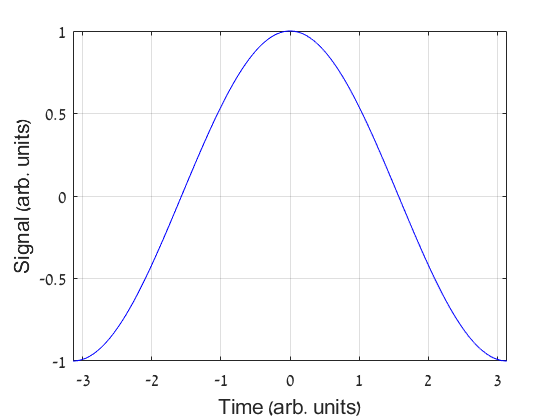
\includegraphics[scale=0.75]{\main/images/chapter_2_example/img_example_2.png}}
	\caption[Another Example Image]{Another Example Image. This image is also labeled internally so we can referenc it throughout the text.}
	\label{fig:cosine-wave}
\end{figure}
\end{document}